\documentclass[11pt]{article}
% motion_header.tex
% include this before the \begin{document} part of your LaTeX source file
%
\usepackage{fourier,ifthen,xspace,amsmath,array}
\usepackage[svgnames, dvipsnames]{xcolor}
\usepackage{graphicx}
\usepackage{siunitx}
\usepackage{xkeyval,calc,moreverb}
\usepackage[breakable,skins]{tcolorbox}
\usepackage{booktabs}
\usepackage{paralist}

% booleans we need
\newboolean{bw}
\setboolean{bw}{false}
\newboolean{solutions}

% counters

\newcounter{problemctr}

% colors

\definecolor{probLineColor}{rgb}{0.2,0.6,0.2}
\definecolor{probLabelColor}{rgb}{0,0,0} % 0.2,0.2,0.7}
\definecolor{probStatementColor}{rgb}{0,0,0}
\definecolor{solColor}{rgb}{0.2,0.6,0.2}

% lengths

\newlength{\probLineWidth} \setlength{\probLineWidth}{1.25pt}
\newlength{\solLineWidth} \setlength{\solLineWidth}{0.5pt}

% oops!
\setlength{\probLineWidth}{0pt}
\setlength{\solLineWidth}{0pt}

% commands

\newcommand{\probdir}{/Users/saeta/Documents/Courses/p24/motion/prob/}
\newcommand{\figdir}{/Users/saeta/Documents/Courses/p24/motion/figs/}
\renewcommand{\probdir}{}
\renewcommand{\figdir}{}
\newcommand{\prob}[2]{% arguments are chapter then problem
  \input{\probdir ch#1/#1P#2}
}

\newcommand{\fig}[2][2]{%
 \vspace*{-.1in}
  \begin{center}%
    \includegraphics[width=#1in]{\figdir#2}
  \end{center}%
}

\newcommand{\SolutionHead}{Solution:}
\newcommand{\theexercise}{}
\newcommand{\PNScolor}[1]{\ifthenelse{\boolean{bw}}{}{\color{#1}}}
\newcommand{\SOL}[1]{\ifthenelse{\equal{#1}{0}}%
  {
\let\solution=\comment
\let\endsolution=\endcomment
\setboolean{solutions}{false}
}%
{\setboolean{solutions}{true}%
\renewenvironment{solution}%
{\par\noindent{\color{solColor}\rule{\linewidth}{\solLineWidth}%
\ifthenelse{\equal{#1}{}}%
{}%
{\par\smallskip\noindent\textbf{\SolutionHead}}}}{}}
}


\newcommand{\val}[2]{\ensuremath{#1~\mathrm{#2}}\xspace}	% number plus unit
\newcommand{\pval}[2]{\ensuremath{\left(#1~\mathrm{#2}}\right)\xspace}
\newcommand{\hval}[2]{\ensuremath{#1$-$\mathrm{#2}}\xspace}
\newcommand{\dg}[1]{\ensuremath{#1^{\circ}}\xspace}
\newcommand{\half}{\ensuremath{\frac{1}{2}}\xspace}
\newcommand{\ux}{\ensuremath{\mathbf{\hat{x}}}\xspace}
\newcommand{\uy}{\ensuremath{\mathbf{\hat{y}}}\xspace}
\newcommand{\uz}{\ensuremath{\mathbf{\hat{z}}}\xspace}
\newcommand{\ur}{\ensuremath{\mathbf{\hat{r}}}\xspace}
\newcommand{\vv}{\ensuremath{v}\xspace}

\newcommand{\xaxis}{$x$ axis\xspace}
\newcommand{\yaxis}{$y$ axis\xspace}
\newcommand{\zaxis}{$z$ axis\xspace}
\newcommand{\xyplane}{$xy$ plane\xspace}
\newcommand{\xzplane}{$xz$ plane\xspace}
\newcommand{\DOT}{\ensuremath{\boldsymbol{\cdot}}}

\newcommand{\bo}{\ensuremath{\boldsymbol{\omega}}\xspace}
\newcommand{\bO}{\ensuremath{\boldsymbol{\Omega}}\xspace}
\newcommand{\VEC}[1]{\ensuremath{\mathbf{#1}}\xspace}
\newcommand{\AU}{\ensuremath{\mathrm{A.U.}}\xspace}
\newcommand{\DB}{\ensuremath{\mathrm{dB}}\xspace}
\newcommand{\degC}[1]{\ensuremath{#1^{\circ}\mathrm{C}}\xspace}


% environments
\newcommand{\problabel}{Problem}
\newenvironment{problem}[1][]%
{
  \begingroup\refstepcounter{problemctr}
  \ifthenelse{\boolean{solutions}}%
    {
      {\vspace*{-10pt}\noindent\PNScolor{probLineColor}%
        \rule[-5pt]{\linewidth}{\probLineWidth}}
    }{}
  \begin{list}{%
      \PNScolor{probLabelColor}\textbf{\problabel\theexercise}%
    }{%
      \setlength{\labelsep}{0pt}%
      \setlength{\leftmargin}{0in}%
      \setlength{\labelwidth}{0pt}%
      \setlength{\listparindent}{0pt}
    }%
    \PNScolor{probStatementColor}%
	\item%
	\ifthenelse{\equal{#1}{}}%
      {}%
      {\textbf{ -- #1}}%
      \quad
}%
{%
  \end{list}\endgroup%
  \PNScolor{black}%
}

\newcommand{\PAGE}[2]{#1-#2\xspace}

\newenvironment{solution}{}{}
\newenvironment{question}{\renewcommand{\problabel}{Question}\begin{problem}}
{\end{problem}\renewcommand{\problabel}{Problem}}

\SOL{1} % show solution

\makeatletter
\newlength\rpLW
\newlength\rpRW
\newlength\rpgap
\newcommand{\rprcent}{0}
\newcommand{\rplcent}{0}
\define@key{rp}{lwidth}{\setlength{\rpLW}{#1}  \setlength{\rpRW}{\columnwidth-#1-\rpgap}}
\define@key{rp}{rwidth}{\setlength{\rpRW}{#1} \setlength{\rpLW}{\columnwidth-#1-\rpgap}}
 \define@key{rp}{lvert}{\def\LeftVerticalCode{#1}}
\define@key{rp}{rvert}{\def\RightVerticalCode{#1}}
\define@key{rp}{gap}{\setlength{\rpgap}{#1}}
\define@key{rp}{rcent}{\def\rprcent{#1}}
\define@key{rp}{lcent}{\def\rplcent{#1}}
\setkeys{rp}{rwidth=2in, lvert=c, rvert=t, gap=0.25in, rcent=0, lcent=0}
\makeatother

\newcommand\rp[3][]{%
  \setkeys{rp}{#1}
  \noindent \parbox[\LeftVerticalCode]{\rpLW}%
  {\ifthenelse{\equal{\rplcent}{0}}%
  {#2}%
  { \begin{center}#2\end{center} }%
  }%
  \hspace*{\rpgap}%
  \parbox[\RightVerticalCode]{\rpRW}%
  {\ifthenelse{\equal{0}{\rprcent}}%
  {#3}%
  {\begin{center} #3 \end{center}}}%
}

\newcommand{\DD}{\ensuremath{d}}		% differential d without leading space
\newcommand{\dd}{\ensuremath{\,\DD}}	% differential d

\newcommand{\deriv}[3][]{\ensuremath{%
	\ifthenelse{\equal{#1}{}}{\frac{\DD #2}{\DD #3}}
	{\frac{\DD^{#1} #2}{\DD #3^{#1}}}}}

\newcommand{\pd}[3][]{\ensuremath{%
	\ifthenelse{\equal{#1}{}}{\frac{\partial #2}{\partial #3}}
	{\partial #2 / \partial #3}}}

\newcommand{\so}{\ensuremath{\qquad\Longrightarrow\qquad}}
\newcommand{\uth}{\ensuremath{\boldsymbol{\hat{\theta}}}\xspace}
\newcommand{\eref}[2][]{%
	\ifthenelse{\equal{#1}{}}%
	{Eq.~(\ref{eq:#2})}%
	{Equation~(\ref{eq:#2})}\xspace}
\newcommand{\cross}{\ensuremath{\times}\xspace}
\newcommand{\into}{\ensuremath{\hat{\otimes}}}	% direction symbols
\newcommand{\outof}{\ensuremath{\hat{\odot}}}
\newcommand{\ds}{\displaystyle}

\newcommand{\xdd}{\ensuremath{\ddot{x}}\xspace}
\newcommand{\thdd}{\ensuremath{\ddot{\theta}}\xspace} % Download this file from physics.hmc.edu/motion/ page
\usepackage{tikz}

\usetikzlibrary{arrows,calc}
                	\tikzset{%
                         every picture/.style={>=stealth'},
                                        vel/.style={->,line width=2pt,color=DarkBlue},
                  force/.style={line width=1.5pt,color=blue,->},
                  coord/.style={color=green!40!black,|->},
                  accel/.style={->,line width=3pt,color=gray},
                  photon/.style={line width=1.5pt,color=DarkRed,decorate,decoration={snake,post length=0.1in}},
                  spring/.style={decorate,decoration={coil,aspect=0.3,segment length=2mm,amplitude=2mm}},
                  traj/.style={dashed, color=gray, line width=1pt}
                }
                
\usepackage{fullpage}
\setlength{\parskip}{6pt}
\setlength{\parindent}{0pt}
\usepackage[margin=1in]{geometry}
\usepackage{graphicx}
\usepackage{enumerate}
\usepackage{marvosym}
\usepackage{amssymb}
\usepackage{wasysym}
\usepackage{gensymb}
\usepackage{mathrsfs}
\usepackage{scrextend}
\usepackage{mathtools}
\usepackage{pgfplots}
\usepackage{xspace}
\usepackage[colorlinks]{hyperref}

% --- style --- %
\renewcommand{\labelenumi}{{ (\alph{enumi})}}
\newcommand{\sand}{\quad \mbox{ and } \quad}
\newcommand{\be}{\begin{enumerate}[a) ]}
\newcommand{\ee}{\end{enumerate}}
\allowdisplaybreaks

% --- making \xi look less awful --- %
\DeclareSymbolFont{CMletters}{OML}{cmm}{m}{it}
\DeclareMathSymbol{\xi}{\mathord}{CMletters}{"18}

% --- math --- %
\newcommand{\Z}{\mathbb{Z}}
\newcommand{\R}{\mathbb{R}}
\newcommand{\C}{\mathbb{C}}
\newcommand{\Q}{\mathbb{Q}}


\newcommand{\Lt}[1]{\mathcal{L}\crb{#1}}
\newcommand{\ilt}[1]{\mathcal{L}^{-1}\crb{#1}}

\newcommand{\pn}[1]{\left( #1 \right)}
\newcommand{\sqb}[1]{\left[ #1 \right]}
\newcommand{\crb}[1]{\left\{ #1 \right\}}
\newcommand{\lra}[1]{\left\langle #1 \right\rangle}
\newcommand{\magn}[1]{\left\lVert #1 \right\rVert}

\newcommand{\pdr}[2]{\frac{\partial #1}{\partial #2}}
\newcommand{\im}[1]{\text{im}\pn{#1}}
\newcommand{\m}[1]{\Z/#1\Z}


\DeclareMathOperator{\proj}{proj}
\newcommand{\vectorproj}[2][]{\proj_{\VEC{#1}}\VEC{#2}}

\newenvironment{amatrix}[1]{%
  \left(\begin{array}{@{}*{#1}{c}|c@{}}
}{%
  \end{array}\right)
}

\newcommand{\spn}[1]{\text{span}\pn{#1}}

\newcommand*\Heq{\ensuremath{\overset{\kern2pt H}{=}}}

\newcommand{\distil}{\sqrt{1-v^2/c^2}}
\newcommand{\distilf}[1]{\sqrt{1-(#1)^2}}
\newcommand{\lorentz}{\frac{1}{\distil}}
\newcommand{\lorentzf}[1]{\frac{1}{\sqrt{1-(#1)^2}}}

\begin{document}

\noindent{\large Problem Set 4, 1 October 2018\hfill Name: \underline{\hspace{3cm}} ,  Section: \underline{\hspace{5mm}} }
\vspace*{0.25in}


\begin{problem}[(P28.10)*]
A total amount of positive charge $Q$ is spread onto a nonconducting, flat, circular annulus of inner radius $a$ and outer radius $b$. The charge is distributed so that the charge density (charge per unit area) is given by $\sigma = k/r^3$, where $r$ is the distance from the center of the annulus to any point on it. Show that (with $V=0$ at infinity) the potential at the center of the annulus is given by
\[
	V = \frac{Q}{8\pi\epsilon_0} \pn{\frac{a+b}{ab}}.
\]
\end{problem}


% Your solution starts here %%%%%%%%%%%%%%%%%%%%%%%%%%%%%%%%%%%%%%%%%%%%%%%%%%
\textbf{Solution:}

% Your solution ends here %%%%%%%%%%%%%%%%%%%%%%%%%%%%%%%%%%%%%%%%%%%%%%%%%%

\clearpage
\begin{problem}[(P28.13)]
On a thin rod of length $L$ lying along the $x$ axis with one end at the origin ($x=0$), as in the figure below, there is a charge per unit length given by $\lambda = kr$, where $k$ is a constant and $r$ is the distance from the origin.
\be
\item Taking the electrostatic potential at infinity to be zero, find $V$ at the point $P$ on the $y$ axis.
\item Determine the vertical component, $E_y$, of the electric field at $P$ from the result of part (a) and also by direct calculation.
\item Why cannot $E_x$, the horizontal component of the electric field at $P$, be found using the result of part (a)?
\item At what distance from the rod along the $y$ axis is the potential equal to one-half the value at the left end of the rod?
\ee
\begin{center}
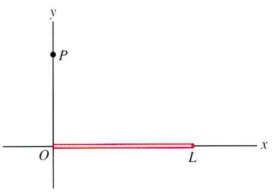
\includegraphics[scale=0.5]{prob2.png}
\end{center}
\end{problem}


% Your solution starts here %%%%%%%%%%%%%%%%%%%%%%%%%%%%%%%%%%%%%%%%%%%%%%%%%%
\textbf{Solution:}

% Your solution ends here %%%%%%%%%%%%%%%%%%%%%%%%%%%%%%%%%%%%%%%%%%%%%%%%%%

\clearpage

\begin{problem}[\P 3.]
In lecture, we calculated the amount of electrostatic energy contained in the interior
electric field of a uniform sphere of radius $R$ and charge density $\rho$. The result was, 
\[
	U = \frac{2\pi\rho^2}{45\epsilon_0}R^5.
\]
For this problem,  complete the calculation by calculating the energy stored in the \textit{exterior}
electric field, and verify that the \textit{total} stored energy matches the work done to assemble the
sphere.
\end{problem}


% Your solution starts here %%%%%%%%%%%%%%%%%%%%%%%%%%%%%%%%%%%%%%%%%%%%%%%%%%
\textbf{Solution:}

% Your solution ends here %%%%%%%%%%%%%%%%%%%%%%%%%%%%%%%%%%%%%%%%%%%%%%%%%%

\clearpage

\begin{problem}[4.]
Consider an infinitely long line of charge with linear charge density $\lambda$ . The line of charge
is parallel to and a distance $d$ above an infinite grounded conducting plane. Sketch the
resulting electric field lines in the half-space above the plane, including any surface
charges. Then using the concepts discussed in lecture, determine the electric field $E(x)$ at
the surface of the plane, as a function of the horizontal distance $x$ from the perpendicular
between the plane and line.
\end{problem}


% Your solution starts here %%%%%%%%%%%%%%%%%%%%%%%%%%%%%%%%%%%%%%%%%%%%%%%%%%
\textbf{Solution:}

% Your solution ends here %%%%%%%%%%%%%%%%%%%%%%%%%%%%%%%%%%%%%%%%%%%%%%%%%%

\clearpage

\begin{problem}[5.]
Consider a hollow conducting sphere that carries a net positive charge $Q$. Next, a second
initially uncharged concentric conducting sphere is brought into proximity with the first
(without touching it). In scenario (a), the second sphere is placed outside the first and left
\textit{ungrounded}. In scenario (b), the second sphere is outside the first and \textit{grounded}. In
scenario (c), the second sphere is \textit{inside} the first and also grounded.
\begin{center}
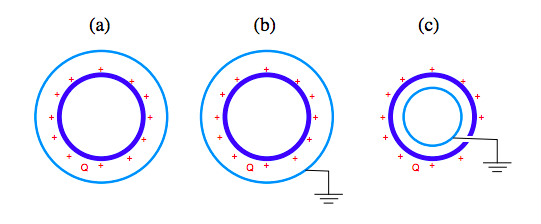
\includegraphics[scale=0.5]{prob5.png}
\end{center}
For all three scenarios, describe the final arrangement of charge on the second sphere and
the electric field (if any) outside the second sphere.
\end{problem}


% Your solution starts here %%%%%%%%%%%%%%%%%%%%%%%%%%%%%%%%%%%%%%%%%%%%%%%%%%
\textbf{Solution:}

% Your solution ends here %%%%%%%%%%%%%%%%%%%%%%%%%%%%%%%%%%%%%%%%%%%%%%%%%%

\clearpage

\begin{problem}[6.]
A cylindrical capacitor is made from two long thin concentric metal cylinders of length $L$
and radii $a$ and $b$. ($L \gg a$ and $a >b$ )
\be
\item Using the definition of capacitance $C =Q V$ ,	calculate the capacitance per unit
length $C /L$ of this configuration.
\item Repeat the capacitance calculation, this time using the stored energy $U = \frac{1}{2}\frac{Q^2}{C}$.
\ee
\end{problem}


% Your solution starts here %%%%%%%%%%%%%%%%%%%%%%%%%%%%%%%%%%%%%%%%%%%%%%%%%%
\textbf{Solution:}

% Your solution ends here %%%%%%%%%%%%%%%%%%%%%%%%%%%%%%%%%%%%%%%%%%%%%%%%%%

\clearpage

\end{document}